\chapter{Parameter Estimation (History Matching/Calibration)}
\label{sec:fepest:parameterEstimation}

\textit{(The terms parameter estimation, history matching and calibration are used synonymously in this document).}

History matching of a model requires completion of the fundamental setup as explained in section \ref{sec:fepest:fundamentalSetup}

After the fundamental setup has been completed, PEST can be advised to perform history matching.
The history matching process targets the estimation of a parameter set that optimally satisfies both the historical observations and - if provided – the prior knowledge. The resulting parameter set is then regarded as a calibrated model.

This section explains the required settings, how the run is commenced and how to interpret the visual feedback during and after the run. Exporting a new FEFLOW model with optimized parameters is the final step.

\section{Required Settings}

\subsection{Optimization Control}

By default, FePEST assumes that history matching is to be performed and applies the respective PEST operation mode accordingly.

Note that the FePEST operation mode is slightly different than the PEST operation mode: If "Estimation" is set, FePEST chooses automatically from "regularization" mode (if the calibration involves Tikhonov regularization) and "estimation" mode (if not). 

A second important option is the NOPTMAX setting found in the termination criteria setting. For calibration purposes, this option must be set to "Number of iterations" and a sufficiently high value (e.g., 30 iterations, which is the default setting).

\subsection{Other settings}

The default settings represent recommendations that are meant to be suitable for a range of optimization processes. Changes might be advised for fine-tuning and trouble shooting. The individual settings will not be explained in detail here, but detailed information is provided in the FePEST help system and the PEST documentation.

\textit{See Section 4.2.2 Control Data of the PEST user manual (5th Edition) for a full discussion of these variables.}

\section{Starting PEST}

Starting the history matching process is done in a sequence of several steps.

\subsection{Pre-Flight Checks}

Before running the model, a sanity check of the PEST setup is recommended. PEST provides several tools (PESTCHEK, TEMPCHEK and INSCHEK) that can be run through the Estimation menu of the FePEST user interface. 

These utilities check the most important files of the PEST setup (the control file, the template file and the instruction file) for errors and warnings. Errors will prevent PEST from running, while warnings are indications for possible problems and give suggestions for improvements of the setup.

\begin{figure}
	\center
	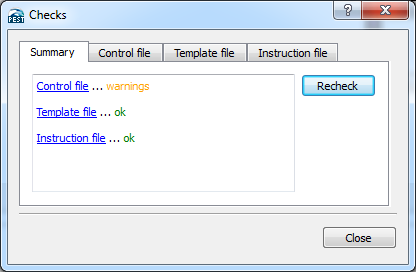
\includegraphics[width=\columnwidth]{figureFundamentalSetup/ChecksDialog.png}
\caption{The Checks utility in the Estimation menu checks the PEST setup for validity and provides suggestions for improvement.}
\label{fig:fepest:ChecksDialog}
\end{figure}

\subsection{Run PEST}

PEST is finally started using the Run button in the toolbar. Usually no change needs to be done to the sequence of steps provided in the upcoming dialog (see Figure \ref{fig:fepest:RunDialogCreateFilesAndRun}).


\begin{figure}
	\center
	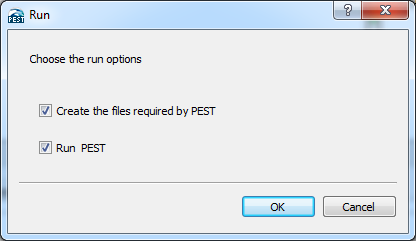
\includegraphics[width=\columnwidth]{figures/RunDialogCreateFilesAndRun.png}
\caption{The Run dialog. Usually all options will be active.}
\label{fig:fepest:RunDialogCreateFilesAndRun}
\end{figure}

The sequence is:

\begin{itemize}
\item	Create the files required by PEST

FePEST generates the required PEST files according to the settings.

\item Recalculate Jacobian Matrix

This option is available if the Jacobian matrix is still available from a former PEST run. Advanced users can choose to deactivate this option to save computational effort.

\item Start PEST

This finally executes PEST itself and commences the actual history matching process. The FePEST windows display the progress of the PEST iteration.

Users experienced in PEST can choose to generate the PEST files without immediately starting the PEST run itself. See also section~\ref{sec:fepest:AdvancedMethods}.

\end{itemize}

It is possible to interrupt (pause) or stop the PEST run. A stopped PEST run can be continued at a later point in time, even if FePEST had to be closed in the meantime. This is useful if the optimization has to be interrupted, e.g., because the computer is turned off. 

\section{Output during PEST Run}

During the PEST run, FePEST reads and analyzes the output of PEST and displays key information in several panels and charts:

\begin{itemize}
\item Output

The primary output of PEST is shown in this window. Users familiar with the output of PEST will find information otherwise omitted in the FePEST output here.

\item Status

Key information on the status of the PEST run is shown in the Status panel.

\begin{figure}
	\center
	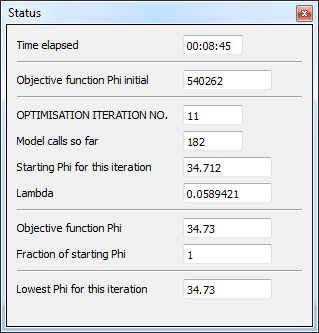
\includegraphics[width=\columnwidth]{figures/statusPanel.png}
\caption{The Status panel contains key information about the progress of the optimization.}
\label{fig:fepest:statusPanel}
\end{figure}

\item Objective Function

The history of the objective function shows the progress of the optimization run and allows identifying the occurrence of problems during the run. Ideally, the function value is shows a continuously falling behavior.

\begin{figure}
	\center 
	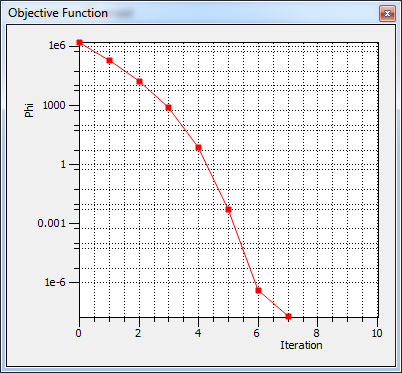
\includegraphics[width=\columnwidth]{figures/ObjectiveFunctionMinimization.png}
\caption{The development of the objective function is shown in the correspondent panel.}
\label{fig:fepest:ObjectiveFunctionMinimization}
\end{figure}

\item Simulated vs. Observed

The panel shows a scatter plot that compares the simulated values with their (observed) reference values.

\item	Simulated vs. Time

A graph shows the time-dependent observations in the model. The measured time series is shown for comparison. This panel is not available for steady-state models.
\end{itemize}

Because the size of the text panels is restricted, they may not contain the complete file. In this case the View… button allows to open the respective file in an external text-editor.

\section{Output after PEST Run}

PEST provides additional statistics after the history matching process. As already during the run, FePEST displays these and other key information in additional panels.

\begin{itemize}

\item	Run Details

PEST journalizes all important information about setup and results of a PEST run into a run record file, which is shown in full in the Run details panel.

\item	Parameter Sensitivities

For all iterations, PEST journalizes composite parameter sensitivities in the sensitivities file, which is shown in full in the Run Details panel. This information can be used to check for example for hypersensitive parameters. The composite sensitivity of a parameter is a measure of the sensitivity of all model outputs for which there are corresponding observations to this parameter. By inference, it is a measure of the information content of the calibration dataset with respect to this parameter.

\item	Observation Sensitivities

PEST writes the observation sensitivities of the last iteration to an observation sensitivities file, which is shown in observation sensitivities.

\item	Residuals

This panel lists the measured and simulated value for each model observation, as well as the difference between these values (the residual). 

The native (non-weighted) residuals allow to identify well or poorly calibrated observations. The weighted residuals (shown separately) are valuable to check for an appropriate choice of observation weights.

The content of this tab is identical to the residuals file created by PEST.

\item	Covariance and Correlation matrix

Covariance and Correlation matrices are only available when not using regularization.

These tables show the covariance and correlation between the parameters, respectively, the latter being normalized to values ranging from 0 (no correlation) to 1 (strong correlation). A color gradient facilitates interpreting the values.

\item	Eigenvectors and Eigenvalues 

Eigenvectors and Eigenvalues are only available when running PEST in estimation mode and not using singular value decomposition.

Each observation contains a certain amount of information that contributes to the identification of the calibrated parameters. Because observations and parameters are often correlated, respectively, the information contributed from a particular observation might overlap with the information that was already provided from a different observation. As a result the number of observations is not necessarily proportional to the combined information of these observations. 

If the covariance matrix undergoes principle component analysis, orthogonal combinations of parameters can be identified, together with the extent to which these combinations have been informed by the calibration process. These combinations are the eigenvectors of the covariance matrix. If a low eigenvalue is associated with this eigenvector, then its post-calibration variability is low. Conversely, if a high eigenvalue is associated with an eigenvector, then its post-calibration variability is high. 

The ratio of highest to lowest eigenvalue is a measure of the extent to which the inverse problem approaches ill-posedness. If this ratio is more than about 5e-7 then the problem can be considered to be ill-posed. Furthermore, unless some kind of regularization is being employed (Tikhonov or SVD) PEST will not be able to solve this inverse problem. Instead its behavior will be numerically unstable, and the objective function may not fall at all.

\end{itemize}

The contents of the text panels can be easily transferred to a spreadsheet program for further processing and visualization.

\textit{See section 5.2: The PEST Run Record and section 5.3: Other PEST Output Files of the PEST user manual (5th Edition) for a full discussion of these output files.}

\section{Export to FEFLOW}

After PEST was able to successfully reduce the objective function to an acceptable level (or another termination criterion was met), it ceases the optimization and FePEST will display a list of resulting parameter values.

To inspect the resulting model more in detail, save it as a new FEM file and open it in FEFLOW.

The found parameter set can also be applied as the initial parameter values, especially if further PEST methods are going to be used.

To return to this dialog at a later point in time, use the Show Results option in the Estimation menu.